%-------------------------------------------------------------------------------
%	CAPITOLO 39
%-------------------------------------------------------------------------------

\chapter{I soci, i parenti}
\index[Personaggi]{Graziani `E Gueran' (contadino)}Il Governo, un contadino\footnote{Era un contadino soprannominato "Il Governo". La famiglia Graziani risponde al soprannome "Gveran".}, non quello che comanda, aveva una barca per caccia insieme ad altri due.\\
\indent Non si trovavano d'accordo sulla caccia.\\
\indent A chi la barca? \\
\indent La segarono in pezzi tre.\\
\\
\centerline{\rule{1.5cm}{0.4pt}}\\
\\
Il \index[Personaggi]{Magnanini}Magnanini aveva in parecchi una biroccia, dovevano dividere. Come fare? Segarono le stanghe, il letto, e dei gavoli delle ruote se ne prese uno a te... uno a me... e così alleviarono le loro fatiche da altri trasporti.\\
\\
\centerline{\rule{1.5cm}{0.4pt}}\\
\\
\index[Personaggi]{Cichinoni}Cichinoni... aveva insieme a suo fratello una casa di due stanze, una sopra l'altra, nelle \index[Luoghi]{Borse (via)}Borse.\\
\indent Dovevano dividere.\\
\indent Cichinoni voleva quella di sotto, perché la voleva guastare come sua legittima proprietà... sulla quale altro nulla può.

\newpage

 \begin{figure}[htb]
    \centering
    %\vspace{-0.7cm}
    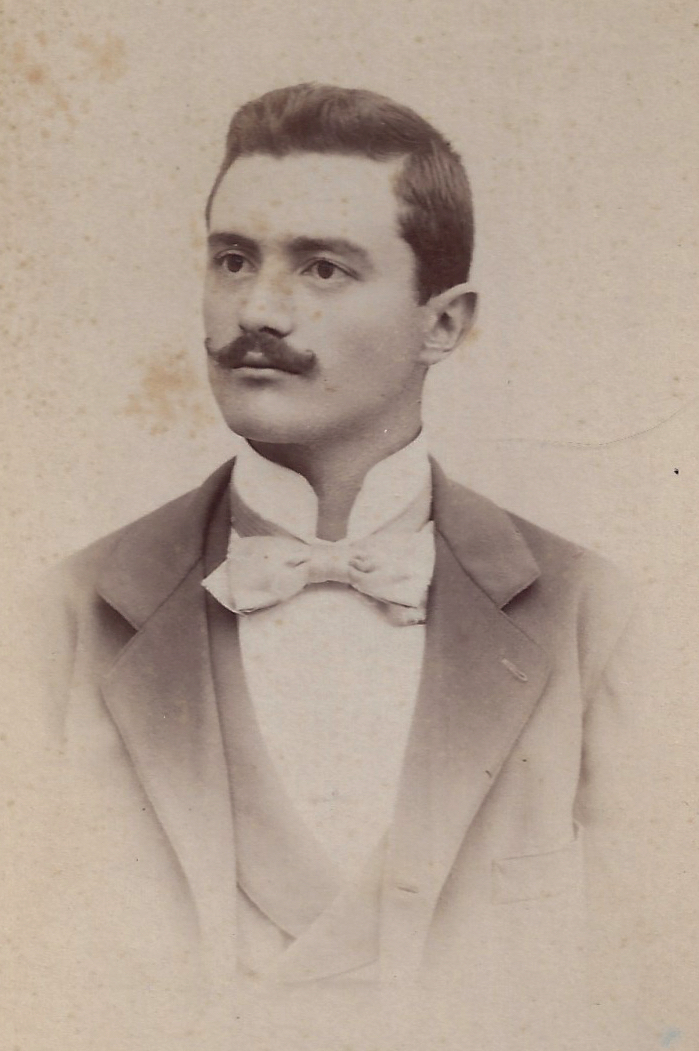
\includegraphics[width=\textwidth]{mingazzigiovane1}
    \caption[Stefano Mingazzi]{\label{fig:mingazzigiovane1}}
    %\vspace{-0.3cm}
\end{figure}